
% Dies ist der "Zentral-Dokument", die verschiedenen Teile k�nnen Sie
% unten einf�gen (s.u.). 
%
 
%[Schritgr��e, Seitenlayout, Papierformat, Satzspiegel, Bindungs-Korrektur-Ma�]
\documentclass[12pt, twoside, a4paper, DIV12, BCOR16mm]{scrartcl}

%L�ndereinstellungen
\usepackage[english, german]{babel}

%Grafiken, erweiterte Kopf- und Fu�zeilen, Seienreferenzvariablen, Listings, erweiterte Symbole,
%deutsche Literatur Formatierung, zeilen-�bergreifende Kommentare, Textmarkierungen
\usepackage{graphicx, fancyhdr, lastpage, listings, wasysym, 
            bibgerm, comment, changebar} 

% weiter evtl. n�tzliche Packages: ifthen, wasysym, changebar, supertabular

%\usepackage{palatino}% weitere Schriftarten

\usepackage[latin1]{inputenc} % Umlaute richtig verarbeiten  
\usepackage[T1]{fontenc}      % Feinheiten im Satz von Umlauten

% Packages, die 'bessere' PDF-Dokumente erzeugen 
\usepackage{ae} 
\usepackage[
        pdftitle={Projektarbeit Verleihsystem}
        bookmarks=true,
        bookmarksnumbered=true, % Verwendete Bookmarks anzeigen
        colorlinks,   % Farbige Links
        linkcolor=black,
        urlcolor=blue,
        citecolor=black]{hyperref}
%\usepackage[dvips]{thumbpdf}

\pagestyle{fancy}

% Legt die Einr�cktiefe der ersten Zeile f�r aller Abs�tze fest. (0:=Abs�tze nicht einr�cken)
\setlength{\parindent}{0pt}  
%\parskip1ex plus0.5ex minus0.5ex   

% Legt die Breite des Randnotizen-Bereichs festlegen (auch �ber BCORxxx konfigurierbar)
%\setlength{\marginparwidth}{25mm}
%\evensidemargin0mm
%\oddsidemargin8mm

% Definiert die Gesamth�he des Textrumpfes f�r alle nachfolgenden Seiten.
\setlength{\textheight}{225mm}
\setlength{\headheight}{13mm}
\setlength{\topskip}{10mm}

% Nummerierungstiefe des Inhaltsverzeichnis 
\setcounter{tocdepth}{2} % auch {3} ist OK aber bitte nicht mehr

% Kopfzeilenformatierung
%\fancyhead[RO,LE]{\small \sffamily Inhalt} 
%\fancyhead[LO,RE]{\small \sffamily Beispiel f�r ein \LaTeX\ Dokument} 


%
% texAbbrev.tex: Einige Abk�rzugen 
%

\newcommand{\ia}{i.\,Allg.\ }
\newcommand{\dht}{d.\,h.\ }
\newcommand{\ua}{u.\,a.\ }
\newcommand{\so}{s.\,o.\ }
\newcommand{\zb}{z.\,B.\ }
\newcommand{\zbdp}{z.\,B.:\ }
\newcommand{\idr}{i.\,d.\,R.\ }
\newcommand{\zt}{z.\,T.\ } 
\newcommand{\zz}{z.\,Zt.\ } 
\newcommand{\igs}{i.\,Ggs.\ } 

\newcommand{\code}{\ttfamily}

\newcommand{\svs}{\vspace*{0.5ex}} 
\newcommand{\myrule}{\ \vspace{1ex} \\ \hrule} 
\newcommand{\figref}[1]{Abb.~\ref{#1}} 
\newcommand{\secref}[1]{Abschnitt~\ref{#1}} 
\newcommand{\mymargin}[1]{\marginpar{\raggedright \footnotesize \sffamily #1}} 

\renewcommand{\topfraction}{0.95}
\renewcommand{\bottomfraction}{0.95}

\newenvironment{trilist}{
    \renewcommand{\labelitemi}{\(\triangleright\)}
    \renewcommand{\labelitemii}{{\bfseries -}}
    \setlength{\partopsep}{0ex plus .5ex minus .5ex} 
    \setlength{\topsep}{-1ex plus .5ex minus .5ex} 
    \setlength{\parskip}{1.2ex plus .5ex minus .5ex}
    \setlength{\itemsep}{0pt plus .5ex minus .5ex}
    \setlength{\parsep}{0pt plus .5ex minus .5ex} 
    \begin{itemize}
    }
   {\end{itemize}}

 % eigene Kommandos laden 


\begin{document} 

\includecomment{comment}
\excludecomment{unsinn1} % ben�tigt das Package "comment". Ein- und Auschalten von Textteilen z.B. Anmerkungen 
\begin{unsinn1} 
Hier steht ein unsinniger Text, welcher aber gl�cklicher Weise nicht angezeigt wird!!!
\end{unsinn1} 

%Titelseite
\begin{titlepage}
\sffamily
\setlength{\tabcolsep}{0mm}
\begin{tabular*}{\textwidth}{l@{\extracolsep\fill}r} 

%\hspace{-0.4cm}
%\includegraphics[width=6cm]{Bilder/logo_welle_en}  % Englische Version des Logos 
\includegraphics[width=5cm]{Bilder/logo_welle_de} % Deutsche Version des Logos

  &
\raisebox{3mm}{
	\begin{tabular}{r}
%\rule{0cm}{0.5cm}
Studiengang Informatik Master\\[0.5mm]
Fakult�t Elektrotechnik und Informatik \\
\end{tabular}}
\end{tabular*}
\setlength{\tabcolsep}{6pt}

\vspace*{4cm}
\begin{center}
\textbf{\Large{Projektarbeit}}\\
\vspace*{1cm}
\textbf{\Huge{Verleihsystem}}\\
\vspace*{2cm}
\end{center}

%\vfill
\vspace{2cm}
\begin{center}

	vorgelegt von:\\[5mm]
{\Large Simon Westphahl} \\[5mm]
{\Large Michael Wydler} \\[5mm]
    \today \\[3cm]
{\normalsize
	\begin{tabular}{rl}
	Betreuerin: 	& Prof. Dr.-Ing. Silvia Keller
	\end{tabular}
}
\end{center}

\end{titlepage}


%Eidesstattliche Erkl�rung
%\begin{newpage}
%\vspace*{\fill}
%\section*{Eidesstattliche Erkl�rung}
%Hiermit versichere ich, die vorliegende Arbeit selbstst�ndig und unter ausschlie�licher Verwendung der angegebenen Literatur und Hilfsmittel erstellt zu haben. Die Arbeit wurde bisher, in gleicher oder �hnlicher Form, keiner anderen Pr�fungsbeh�rde vorgelegt und auch nicht ver�ffentlicht.\\

%\vspace{3cm}
%\begin{tabular*}{\textwidth}{c@{\extracolsep\fill}cc}
%\cline{1-1}
%\cline{3-3}
%\\
%\ \ \ \ \ \ \ \ \ Unterschrift\ \ \ \ \ \ \ \ \ \ & & \ \ \ \ \ \ \ \ \ Ort, Datum\ \ \ \ \ \ \ \ \ \\
%\end{tabular*}
%\end{newpage}


%Vorwort, Zusammenfassung(Abstract), Danksagung(Acknowledgements)
\begin{newpage}
\vspace*{\fill}
\section*{Vorwort}
Zusammenfassung / Abstract\\
Danksagung / Acknowledgements\\
Motivation usw. geh�ren hierher.\\
\end{newpage}


\newpage


\tableofcontents 

%Seitenzahl und Kapitelname in der Kopfzeile anzeigen
%\fancyhead[RO,LE]{\small \sffamily  \thepage}
%\fancyhead[LO,RE]{\small \sffamily \leftmark}

% f�gen Sie hier die einzelnen Teile (z.B. Kapitel) ein.  

\section{Einleitung \label{Einleitung} }
Die ist ein kurzes Beispiel zu \LaTeX , es soll keine Einf�hrung sein -- Sie
k�nnen diese Datei aber als Ausgangspunkt f�r Ihr eigenes Werk nehmen.  Eine
Einf�hrung in \LaTeX\ finden Sie in den Tutorials: latexTutorial1.pdf
latexTutorial2.pdf. 

Wenn ein Dokuement einen \LaTeX-Fehler enth�lt, erwartet das Programm eine
Eingabe. Meist ist es sinnvoll, nur den Buchstaben 'q' einzugeben. Dies schaltet
\LaTeX\ auf stumm. Anschlie�end kann man in der formatierten Datei meist erkennen,
wo sich der Fehler befindet. Genauers entnimmt man der Datei {\code <name>.log}.  

Eine Rechtschreibpr�fung f�r \LaTeX-Dokumente gibt es ebenfalls. Unter Unix/Linux
\zb {\code ispell -C -Tlatin1 -t -d ngerman Einleitung.tex} (wenn sie mit UTF-8
Codierung arbeiten muss der 2. Parameter {\code -Tutf-8} lauten).


\subsection{Problemstellung \label{Problemstellung} } 

Ein g��eres Dokument\footnote{Fu�noten sind ebenfalls problemlos m�glich.} zerlegt man am besten in ein "'Zentral-Dokument"' und die
einzelnen Kapitel bzw. Abschnitte (s.~Datei {\code Thesis.tex}. Der \LaTeX\
"'Source Code"' wird �bersetzt in das DVI-Format. Das DVI-File kann dann auf dem
Bildschirm angezeigt und/oder gedruckt werden oder in ein anderes Format gewandelt
werden (\zb PostScript, PDF, HTML).

Befehle (Bsp.):
\begin{verbatim}
> latex Thesis.tex
> dvips Thesis.dvi 
> dvipdf Thesis.dvi
> ghostview Thesis.ps 
> ps2pdf Thesis.ps Thesis.pdf 
> latex2html Thesis.tex 
\end{verbatim} 

Alternativ kann der \LaTeX\ "'Source Code"' (ohne Umwege �ber das DVI-Format) direkt in das PDF-Format �bersetzt werden:
\begin{verbatim}
> pdflatex Thesis.tex
\end{verbatim} 

Das Literaturverzeichnis erstellt man am besten mit dem Programm
BibTeX. Voraussetzung ist nat�rlich, dass man eine BibTex-Datei mit den
Literatur-Eintr�gen erstellt hat (in diesem Fall: Literatur.bib). 
\begin{verbatim}
> latex Thesis.tex
> bibtex Thesis
> latex Thesis.tex
> latex Thesis.tex
\end{verbatim} 

Hier folgen noch ein paar Beispiele f�r \LaTeX-Konstruktionen bzw.\ selbst definierte
Kommandos Kommandos Kommandos Kommandos Kommandos: 

\paragraph{Querverweis:} Dies ist ein Querverweis auf \secref{Zielsetzung} (das Kommando
\verb+\secref{}+ ist von mir in {\code Abkuerzugen.tex} definiert). 

\paragraph{Literaturhinweise:} Ein Literaturhinweis
entsteht durch \cite{mandl99} bzw. durch \cite{sing00, zeller02,edwards00}. Das
Kommando \verb+\cite{...}+ ist bereits in \LaTeX\ definiert. Die Quellen-Angaben
schreiben Sie in eine Datei mit der Endung \verb+.bib+, n�heres s.~Tutorial. 

Die verschiedenen Kommandos in der Datei {\code Abkuerzugen.tex} \mymargin{nur am
Rande, bei Bedarf} ergeben \ua folgende Abk�rzungen; \ia und \zb und \dht und \zz
sowie eine Randbemerkung.

\begin{itemize} 
   \item  eine Aufz�hlung
   \item  noch ein Punkt 
   \item  bla
\end{itemize} 
\LaTeX und Emacs: Abk�rzungen machen das Leben leichter. Einige Definitionen finden
sich in der Datei {\code Abkuerzugen.emacs}. So bewirkt \zb die Eingabe von
\verb+bgit<space>+, dass Emacs die folgenden drei Zeilen einf�gt: 
\begin{verbatim}
\begin{itemize} 
   \item 
\end{itemize}  
\end{verbatim} 
Die Datei {\code Abkuerzugen.emacss} muss von Emacs geladen
werden, am besten automatisch durch einen Eintrag in {\code .emacs},{\code
  .gnu-emacs} oder{\code .gnu-emacs-custom} je nach Installation \smiley.
\begin{verbatim} 
  (if (file-readable-p "~/etc/TeX/Abkuerzugen.emacs")
      (read-abbrev-file "~/etc/TeX/Abkuerzugen.emacs")) 
\end{verbatim} 

bla bla bla bla bla bla bla bla bla bla bla bla bla bla bla bla bla
bla bla bla bla bla bla bla bla bla bla bla bla bla bla bla bla bla
bla bla bla bla bla bla bla bla bla bla bla bla bla bla bla bla bla
\begin{enumerate} 
   \item  eine Aufz�hlung nummeriert 
   \item  Aufz�hlungen k�nnen auch geschachtelt werden \ldots
   \item  bla
\end{enumerate} 

bla bla bla bla bla bla bla bla bla bla bla bla bla bla bla bla bla
bla bla bla bla bla bla bla bla bla bla bla bla bla bla bla bla bla
bla bla bla bla bla bla bla bla bla bla bla bla bla bla bla bla bla
bla bla bla bla bla bla bla bla bla bla bla bla bla bla bla bla bla

\begin{table}[htb] 
\caption{Eine Tabelle hat (manchmal) eine �berschrift} 
\begin{center}
\begin{tabular}{|rc|}           \hline
eine Tabelle & zweite Spalte \\ \hline \hline 
  a          & b             \\ 
  ccc        & ddd           \\ 
 aber        & ohne          \\ 
 Buch        & geht's nicht  \\ \hline 
\end{tabular} 
\end{center}
\end{table} 

bla bla bla bla bla bla bla bla bla bla bla bla bla bla bla bla bla
bla bla bla bla bla  


\subsection{Zielsetzung \label{Zielsetzung} } 

bla bla bla bla bla bla bla bla bla bla bla bla bla bla bla bla bla
bla bla bla bla bla bla bla bla bla bla bla bla bla bla bla bla bla
bla bla bla bla bla bla bla bla bla bla bla bla bla bla bla bla bla

\begin{figure}[htbp]
\centering 
 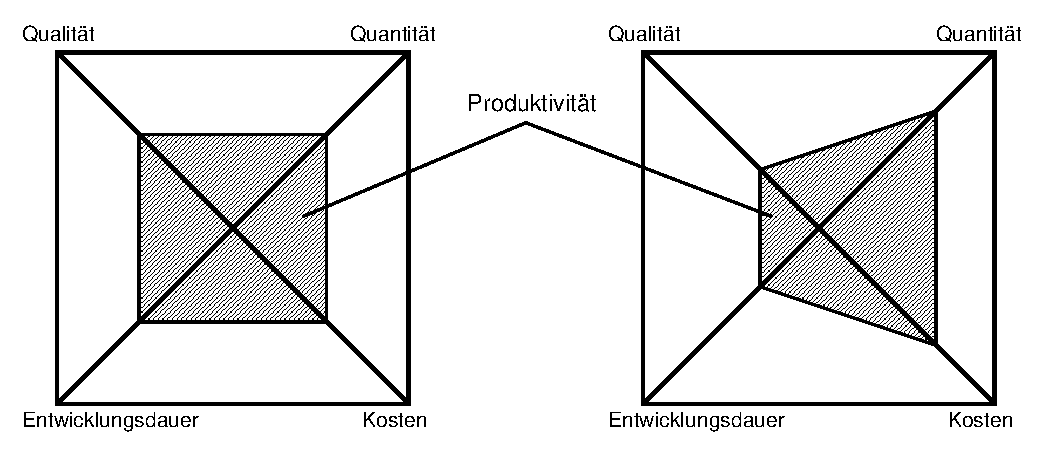
\includegraphics[width=0.8\textwidth]{Bilder/magicSquare} 
 \caption{Das magische Quadrat der konkurrierenden Ziele (als encapsulated
          postscript)  \label{magicSquare}}
\end{figure}
Auf Abbildungen kann nat�rlich auch referenziert werden \zb durch
"'\figref{magicSquare} auf Seite~\pageref{magicSquare}"'. Dies setzt allerdings
voraus, dass man ein Label definiert hat (\zb \verb+\label{magicSquare}+). Der Befehl
\verb+\figref{..}+ ist nicht von \LaTeX\ definiert sondern in der Datei {\code
Abkuerzugen.tex}.  Hier sieht man auch, wie man Anf�hrungszeichen schreibt \ldots
  
bla bla bla bla bla bla bla bla bla bla bla bla bla bla bla bla bla
bla bla bla bla bla bla bla bla bla bla bla bla bla bla bla bla bla
bla bla bla bla bla  

\newpage
\subsection{Noch ein paar Anmerkungen \label{Anmerkungen}} 

bla bla bla bla bla bla bla bla bla bla bla bla bla bla bla bla bla
bla bla bla bla bla bla bla bla bla bla bla bla bla bla bla bla bla

\begin{comment} 
\cbstart 
\ \vspace{0.5ex}
\hrule 
\ \vspace{0.5ex}

Dieser Abschnitt erscheint nur, wenn der Befehl \verb+\includecomment{comment}+ in
der \LaTeX -Hauptdatei steht.  Mit einem \verb+%+ -Zeichen kann er auskommentiert
werden. Dann verschwindet dieser Absatz aus dem Dokument.

Kommentar-Bereiche sind praktisch um Textteile im Dokument "'parken"' zu k�nnen. Bei
Bedarf kann man die Teile sichtbar bzw.\ unsichtbar schalten.  Der graue Balken am
Rand wird durch die Befehle \verb+\cbstart+ und \verb+\cbend+ erzeugt. Dazu muss das
Package \verb+changebar+ geladen werden. 
\ \vspace{0.5ex}
\hrule 
\ \vspace{0.5ex}\cbend
\end{comment} 

bla bla bla bla bla bla\footnote{Fu�noten sind ebenfalls problemlos m�glich.} bla bla
bla bla bla bla bla bla bla bla bla bla bla bla bla bla bla bla bla bla bla bla bla
bla bla bla bla bla bla bla bla bla bla bla bla bla bla bla bla bla bla bla bla bla
bla bla bla bla bla bla



 
\section{Stand der Technik \label{StandDerTechnik} }

\include{Methode}
\include{Ergebnisse}
\section{Zusammenfassung und Ausblick \label{ZusammenfassungUndAusblick} }


\begin{comment} 
\nocite{coulouris00, coulouris02} 
\end{comment} 

\addcontentsline{toc}{section}{Literatur} 
\bibliographystyle{gerplain} 
\bibliography{Literatur} 

\end{document} 


